\section{PhoenixSim}

\begin{figure}[H]
\caption{Vista General PhoenixSim. Fuente \cite{Chan2011}}
\centering
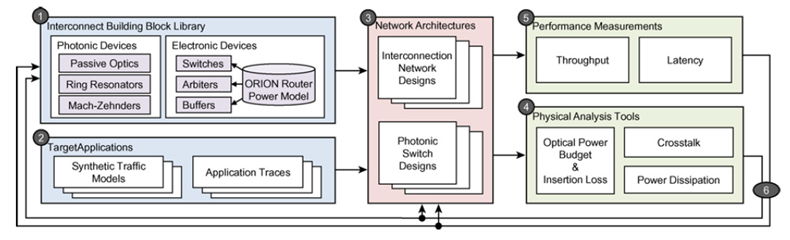
\includegraphics[width=1.0\textwidth,natwidth=790,natheight=240]{figs/overview.png}
\label{fig:phoenix_ovw}
\end{figure}

\subsection{Dispositivos de Interconexión}
\subsubsection{Electrónicos}

\paragraph{Router Electrónico}~\\
\begin{itemize}
\item Puerto de Entrada (InPort)
\item Entramado de comunicación (Crossbar)
\item Controlador (Arbiter)
\end{itemize} 

\subsubsection{Fotónicos}
La caracterización  de los dispositivos de PhoenixSim abstrae las características físicas más importantes de los elementos fotónicos (capítulos \ref{ch:intro} y \ref{ch:rr}) sin perder la presición de sus resultados y sin necesidad de realizar una simulación FDTD completa. 

Al usar sólo las características más relevantes, se pueden emplear como componentes de las diferentes redes al mismo tiempo que se mantiene el rendimiento de la simulación a nivel de sistema.

\paragraph{Pasivos}~\\
\begin{itemize}
\item Guía de onda

Cables óptivos con los que se conectan los demás dispositivos fotónicos. Exhiben 
pérdidas de propagación principalmente debido a las imperfecciones en el proceso
de fabricación y a rugosidades en las paredes de la misma.
La abstracción de su funcionamiento está basada en 3 parámetros \cite{Chan2011} 
(ver Tabla \ref{tb:wg_params}).

\begin{figure}[H]
\caption{Caracterización: Guía de Onda.}
\centering
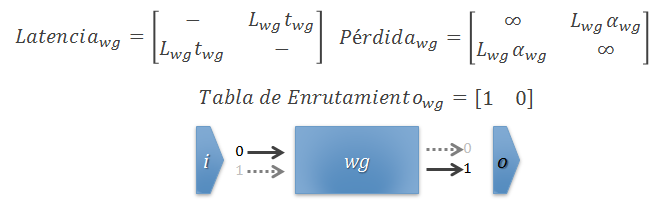
\includegraphics[width=0.9\textwidth,natwidth=665,natheight=200]{figs/wg.png}
\label{fig:phoenix_wg}
\end{figure}

\begin{table}[H]
\centering
\begin{tabular}{|c|c|c|}
\hline
Descripción &  Nombre Parámetro & Abv. \\
\hline
Longitud & $Length$ & $L_{wg}$ \\
Latencia & $LatencyRate_Line$ & $t_{wg}$ \\
Pérdidas por Propagación & $PropagationLoss$ & $\alpha_{wg}$ \\
\hline
\end{tabular}
\caption{Caracterización Guía de Onda.}
\label{tb:wg_params}
\end{table} 

\item Guía de onda doblada

\item Cruce de guías de onda
\begin{figure}[H]
\caption{Caracterización: Cruce de Guía de Onda.}
\centering
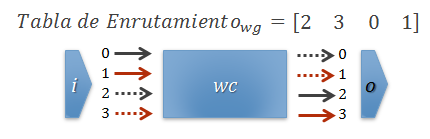
\includegraphics[width=0.6\textwidth,natwidth=430,natheight=139]{figs/wgcross.png}
\label{fig:phoenix_wgc}
\end{figure}

\end{itemize}

\paragraph{Activos (basados en anillos resonadores \ref{ch:rr})}~\\
\begin{figure}[H]
\caption{(a). Cambio de estado de resonancia on-off
al aplicar un voltaje Fuente \cite{hendry2011time}. (b). Caracterización: Anillo Resonador.}
\centering
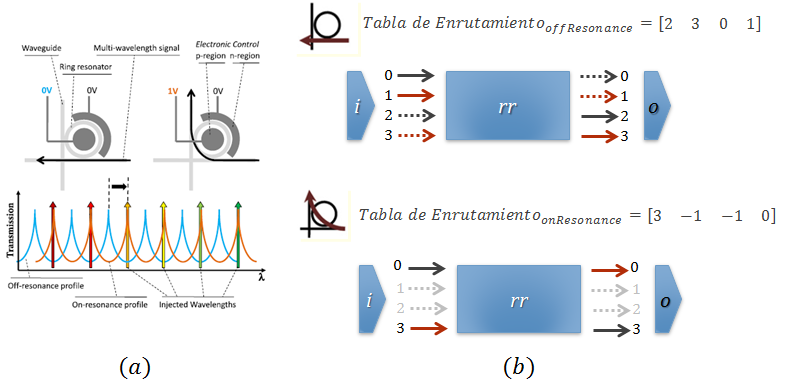
\includegraphics[width=1.0\textwidth,natwidth=800,natheight=390]{figs/rr.png}
\label{fig:phoenix_wgc}
\end{figure}

\begin{itemize}
\item Filtros
\item Switches de banda ancha
\item Moduladores
\item Detectores
\end{itemize}  




\subsection{Benchmarks}
\subsubsection{Modelos de Patrones Sintéticos}
All2All permite probar que todas las rutas de comunicación entre los nodos sean accesibles. Esto permite evaluar el peor caso de pérdida por inserción en la red fotónica \cite{Manual}.


\paragraph{Pruebas de Memoria DRAM}~\\
Las pruebas sobre la memoria están divididas en 3 según la característica que se desee analizar: 
\begin{itemize}
\item One2One comunica un procesador y un módulo de memoria DRAM. Esto premite probar la latencia de los accesos a memoria cuando no hay carga en la red (zero-load latency).
\item One2All comunica un procesador hacia todos los módulos de memoria DRAM, con lo que se puede determinar la accesibilidad de estos.
\item All2One prueba el mecanismo de contención al generar un patrón de comunicación de estrés donde todos los procesadores acceden a un solo módulo de memoria.
\end{itemize} 

\subsubsection{Modelos de Aplicaciones Reales}
\paragraph{Transformada rápida de Fourier (FFT)}~\\

Está dividido en las etapas del algoritmo de Cooley-Turkey. La etapa principal es la que toma el mayor tiempo, 
Los tiempos de cada etapa deben ser pasados como parámetros de la simulación. Los valores por defecto incluidos en el texit{textbed} de PhoenixSim fueron obtenidos de la caracterización  dada por Frigo y Johnson \cite{benchFFT} y usa 8 núcleos de procesamiento. 

\subsection{Herramientas de Medición y Análisis}

